\chapter{Background} \label{chap:background}

In this chapter we introduce general concepts to better understand the design and implementation details of \projName.
Firstly, we introduce the hardware, software and programming frameworks that we leverage, and then the medical technicalities regarding the data we use and the processing we make of it.
In \S\ref{sec:background:tech}, we cover technical aspects exploited in the remaining of this work, specifically: we descrive the concept of Trusted Execution Environment, the operating principles of Intel SGX and Spark, and lastly we present two key frameworks developed by the \textit{Large Scale Data \& Systems}~\cite{lsds} group at the Imperial College London, \textsc{SGX-LKL} and \sgxspark.
In \S\ref{sec:background:med}, we describe the specificities of the data streams that \projName has to deal with from the medical domain, how this data streams are obtained, together with the required processing that our system allows to offload on an untrusted cloud provider, and how this processing can be useful in a real use case.

\section{Technical Background} \label{sec:background:tech}

\subsection{Trusted Execution Environments and Intel SGX}
A \emph{trusted execution environment (TEE)} is an isolated area of a main processor that provides code and data therein contained with confidentiality and integrity guarantees~\cite{tee-globalplatform}. 
Confidentiality refers to preventing unauthorized parties from accessing sensitive information and integrity to ensuring that sensitive code and data is not tampered with.
An application developed to run and deployed in a TEE is called a \emph{Trusted Application (TA)}.
%The main CPU vendors have already implemented Trusted Execution Environments in their commodity CPUs.
Trusted Execution Environments have already been available for several years in the main CPU vendors' commodity CPUS.
\arm \tz has been part of \arm's architecture since v6 for Cortex-A processors (2012) and v8 for Cortex-M (2018).
Intel\textregistered\xspace \textsc{Software Guard Extensions (SGX)} were introduced with the sixth generation of Intel's processors codename \textit{Skylake} in 2015.

In comparison with \arm \tz, \textsc{Intel SGX} include a remote attestation protocol, support multiple trusted applications on the same CPU, its SDK is easier to program with, and there is a greater variety of programming frameworks to develop SGX-based TAs.
Most importantly, all the major Infrastructure-as-a-Service (IaaS) providers (Google~\cite{gceskylake}, Amazon~\cite{amazonskylake}, IBM~\cite{ibm-sgx}, Microsoft~\cite{azureconfidential}) are nowadays offering nodes with SGX processors.
For these reasons, \textsc{Intel SGX} is our chosen hardware solution to deploy \projName in.
\begin{wrapfigure}{r}{.5\textwidth}
    \centering
    \resizebox{\linewidth}{!}{
\begin{tikzpicture}

    % Main outline
    %\draw[fill=green1] (0,0) rectangle (10, 1) node[pos=.5] {Privileged System Code, OS, VMM};
    \draw[fill=gray!10] (0, 0) rectangle (10, 8.5);

    % Unsecure Part
    \node[align=center] at (2.25, 7.5) {\textbf{Untrusted Code}};
    \draw[dashed, fill=white] (0.5, 0.5) rectangle (4, 7.0);
    \node at (1.25, 1.25) {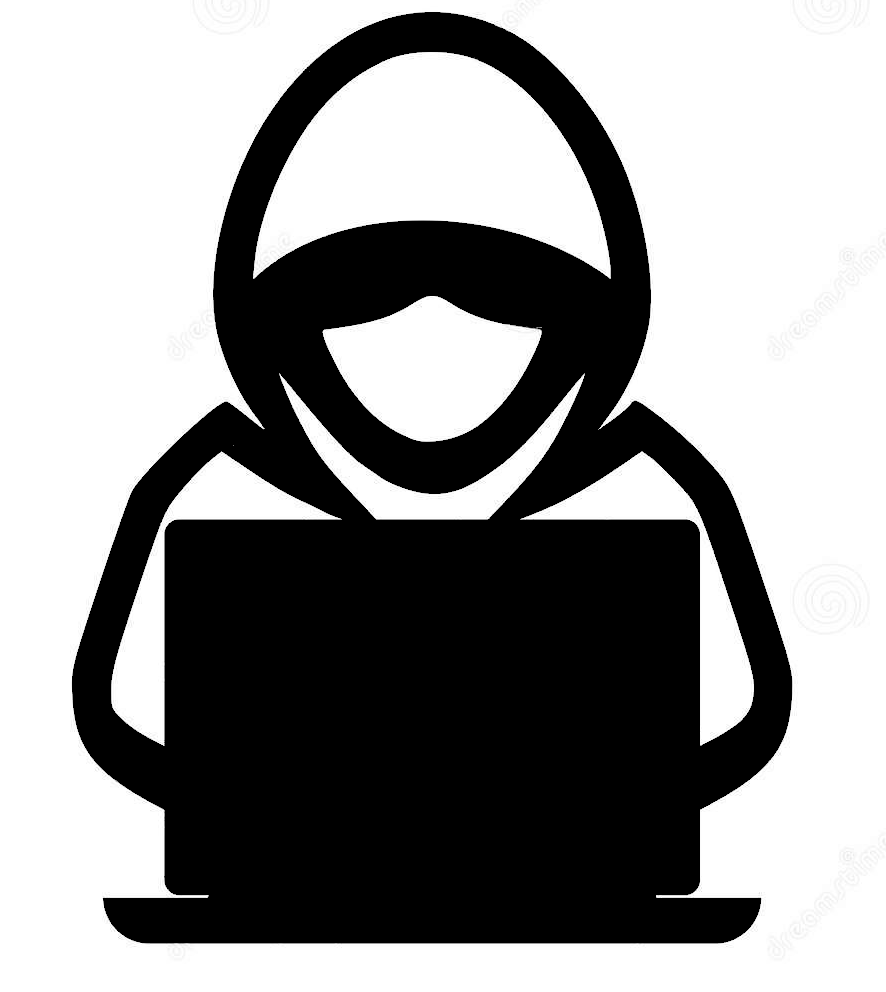
\includegraphics[width=25pt]{img/hacker.png}};
    \draw[->,thick, decorate,decoration={snake, post=lineto, post length=1mm}] (2.25, 6.5) -- (2.25, 5.75) node[pos=.3,anchor=west] {\blackcircled{1}};
    \node[align=center] at (2.25, 5.5) {\texttt{Create Enclave}};
    \draw[->,thick, decorate,decoration={snake, post=lineto, post length=1mm}] (2.25, 5) -- (2.25, 4) node[pos=.5,anchor=west] {\blackcircled{2}};
    \node[align=center] at (2.25, 3.5) {\texttt{Call Trusted} \\ \texttt{Function}};
    \draw[->,thick, decorate,decoration={snake, post=lineto, post length=1mm}] (2.25, 3) -- (2.25, 2) node[pos=.3,anchor=west] {\blackcircled{7}};
    \draw[->, very thick] (4, 5.25) -- (5.5, 5.25) node[pos=.5,anchor=south] {\blackcircled{3}};

    % Secure Part
    \node[align=center] at (7.75, 7.5) {\textbf{Trusted Code}};
    \draw[fill=white,pattern=north west lines,pattern color=gray!50] (6, 0.5) rectangle (9.5, 7.0);
    \node at (8.75, 1.25) {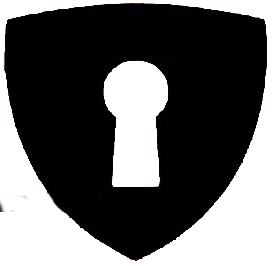
\includegraphics[width=25pt]{img/intel-sgx.png}};
    \node[align=center] at (5.55, 6.5) {\small{Call} \\ \small{Gate}};
    \draw[fill=gray!80] (5.5, 5.5) rectangle (6, 6.0);
    \draw[fill=gray!80] (5.5, 5.0) rectangle (6, 5.5);
    \draw[fill=gray!80] (5.5, 4.5) rectangle (6, 5.0);
    \draw[rounded corners, dashed, fill=white] (6.5, 2.5) rectangle (9, 5.75);
    \draw[->, very thick] (5.75, 5.25) -- (6.75, 5.25) node[pos=.5,anchor=south] {\blackcircled{4}};
    \node[align=center] at (7.75, 5.25) {\texttt{Execute}};
    \draw[->,thick, decorate,decoration={snake, post=lineto, post length=4mm}] (7.75, 5) -- (7.75, 3.25) node[pos=.5,anchor=west] {\blackcircled{5}};
    \node[align=center] at (7.75, 3) {\texttt{Return}};
    \draw[->, very thick] (6.75, 3) -- (4, 3) node[pos=.6, anchor=south] {\blackcircled{6}};
\end{tikzpicture}}

    \caption{\textsc{Intel SGX} execution workflow.\label{fig:sgx-principles}}
\end{wrapfigure}
Intel \textit{Software Guard eXtensions} are a set of new instructions and memory access changes added to Intel's architecture.
These extensions enable applications to create hardware-protected containers in their address space, referred to as \emph{enclaves}.
An enclave provides confidentiality and integrity even in the presence of malicious privileged software such as virtual machine monitors (VMM), BIOS or operating systems (OS)~\cite{McKeen2013}. 
At initialization time, the code and data is free for inspection and, once loaded to the enclave, the latter is measured (via hashing) and sealed. 
An application using an enclave identifies itself through a remote attestation protocol and, once verified, interacts with the protected region through a call gate mechanism.
The application can also verify that its secure code is running in a genuine enclave using the same attestation protocol via platform specific keys. %The basic mechanisms of SGX are depicted in Figure~\ref{fig:sgx-principles}.

Services using SGX divide its source code in an untrusted and a trusted part.
The former deployed outside the enclave and the latter inside.
Figure~\ref{fig:sgx-principles} breaks down the typical execution workflow of SGX services.
After the initial attestation protocol, code in the untrusted region creates an enclave and securely loads trusted code and data inside (Figure-\ding{202}). 
Whenever this untrusted code wants to make use of the enclave, it makes a call to a trusted function (Figure-\ding{204}) that gets captured by the call gate mechanism and, after performing sanity and integrity checks (\ding{205}), gets executed (\ding{206}), the value returned (\ding{207}) and the untrusted code can resume execution (\ding{208}).
It is important to stress that the security perimeter is kept at the CPU package and, as a consequence, all other software including privileged software or even other enclaves are prevented from accessing code and data located inside the enclave. 
In particular, the systems' main memory is left untrusted and the traffic between CPU and DRAM over the protected address range is managed by the \textit{Memory Encryption Engine (MEE)}~\cite{Gueron16}.
% TODO: should we mention SGX's main drawbacks or vulnerabilities?

\subsection{Spark and Spark Streaming}
\textsc{Apache Spark} is a cluster-computing framework to develop scalable, fault-tolerant, distributed applications. 
It builds on RDDs, resilient distributed datasets~\cite{McKeen2013}, a read-only collection distributed over a cluster that can be rebuilt if one partition is lost. 
It is implemented in \textsc{Scala} and provides bindings for \textsc{Python}, \textsc{Java}, \textsc{SQL} and \textsc{R}. 
\textsc{Spark Streaming}~\cite{Zaharia2012} is an extension of Spark's core API that enables scalable, high-throughput, fault tolerant stream (mini-batch) processing of data streams~\cite{ZahariaDStreams2012}.
\projName leverages Spark Streaming to perform file-based streaming, by monitoring a filesystem interface outside the enclave and processing new files as they are loaded.
In particular, and as detailed later in Chapter \ref{chap:implementation}, \projName uses the \textit{Discretized Streams} API~\cite{spark-streaming-documentation}.

\subsection{SGX-LKL and SGX-Spark}
Developed at the \textit{Large Scale Data \& Systems Group (LSDS)}~\cite{lsds} at the \textit{Imperial College London}, \textsc{SGX-LKL}~\cite{sgx-lkl} is a library OS to run unmodified Linux binaries inside enclaves.
It provides support for complex applications and managed runtimes enabling in-enclave user-level threading, signal handling, and paging.
Namely, it allows the execution of a full \textit{Java Virtual Machine (JVM)} inside an enclave. 
This feature enables the deployment of Spark, and Spark Streaming applications to leverage critical computing inside Intel SGX with minimal to no modifications to the application's code. 
\begin{wrapfigure}{r}{.5\textwidth}
    \centering
    \vspace{-21pt}
    \resizebox{.4\textwidth}{!}{
\begin{tikzpicture}
    % Colors definition: latexcolor.com
    \definecolor{ashgrey}{rgb}{0.7, 0.75, 0.71}
    \definecolor{x11gray}{rgb}{0.75, 0.75, 0.75}

    
    % Main outline
    \draw[fill=gray!10] (0,0) rectangle (3, 4);

    % First Layer
    % Shared Memory
    \draw[fill=white] (0.25, 0.25) rectangle (2.75, 0.5) node[pos=.5] {\tiny SHM};
    \node at (0.45, 0.375) {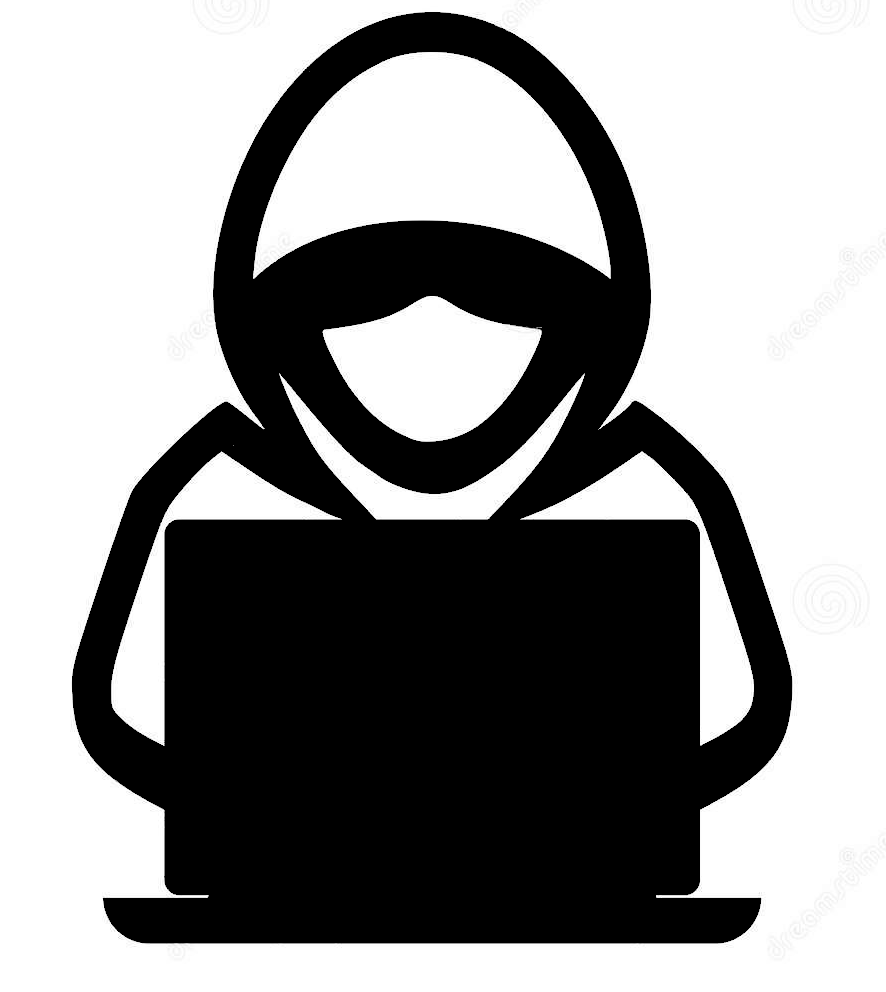
\includegraphics[width=5pt]{img/hacker.png}};

%    \draw[fill=white] (0.25, 0.25) rectangle (1.45, 0.825) node[pos=.5] {\tiny{OS}};;
%    \node at (0.45, 0.45) {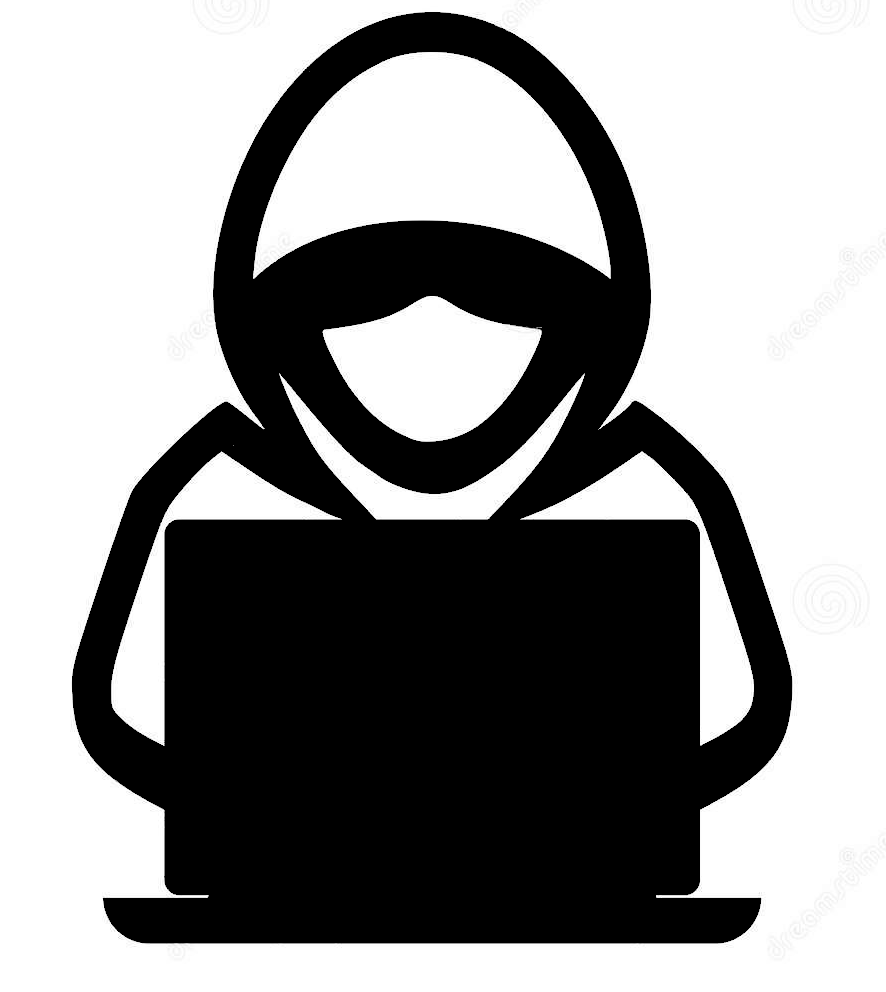
\includegraphics[width=8pt]{img/hacker.png}};
%    \draw[fill=white, pattern=north west lines,pattern color=gray!50] (1.55, 0.25) rectangle (2.75, 0.825) node[pos=.5] {\tiny{SGX}};
%    \node at (2.55, 0.45) {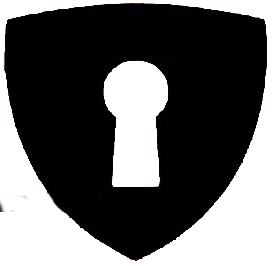
\includegraphics[width=8pt]{img/intel-sgx.png}};

    % Second Layer
    \draw[fill=white] (0.25, 0.6) rectangle (1.45, 1.55) node[pos=.5, xshift=2pt, yshift=3pt, align=center] {\tiny{Spark} \\[-9pt] \tiny{Worker}};
    \node at (0.45, 0.8) {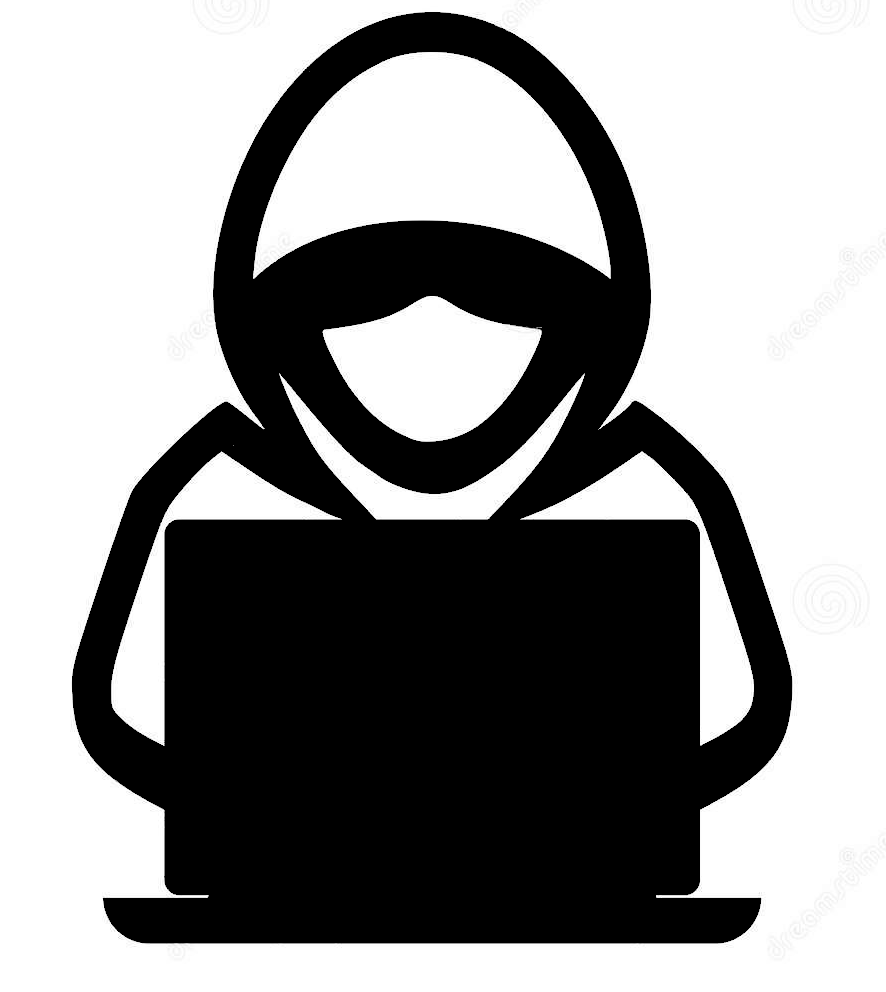
\includegraphics[width=8pt]{img/hacker.png}};
    \draw[fill=white, pattern=north west lines,pattern color=gray!50] (1.55, 0.6) rectangle (2.75, 1.55) node[pos=.5, xshift=-3pt, yshift=3pt, align=center] {\tiny{Worker} \\[-9pt] \tiny{Enclave}};
    \node at (2.55, 0.8) {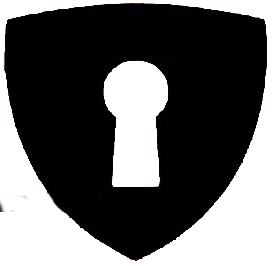
\includegraphics[width=8pt]{img/intel-sgx.png}};

    % Third Layer
    \draw[fill=white] (0.25, 1.65) rectangle (1.45, 3.4);
    \node[align=center] at (0.85, 2.65) {\tiny{Driver} \\[-10pt] \tiny{\&} \\[-10pt] \tiny{App Entry} \\[-10pt] \tiny{Point}};
    \node at (0.45, 1.85) {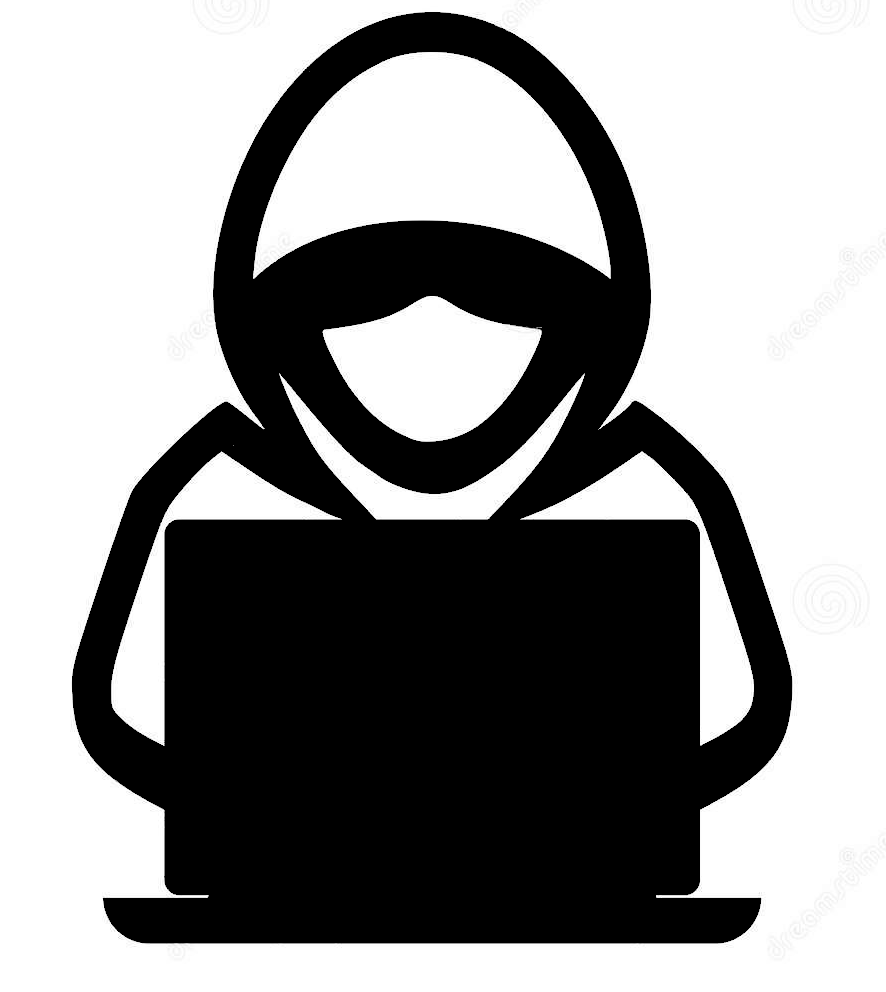
\includegraphics[width=8pt]{img/hacker.png}};
    \draw[fill=white, pattern=north west lines,pattern color=gray!50] (1.55, 1.65) rectangle (2.75, 3.4);
    \node[align=center] at (2.15, 2.85) {\tiny{Driver} \\[-10pt] \tiny{Enclave}};
    \node at (2.55, 1.85) {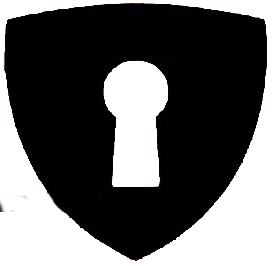
\includegraphics[width=8pt]{img/intel-sgx.png}};
    % Spark Tasks
    \draw[fill=white] (1.6, 2.1) rectangle (1.95, 2.4) node[pos=.5] {\tiny{T$1$}}; 
    \node at (2.15, 2.25) {\tiny{$\cdots$}};
    \draw[fill=white] (2.35, 2.1) rectangle (2.7, 2.4) node[pos=.5] {\tiny{T$N$}}; 

    % Spark Master
    \draw[fill=white] (0.25, 3.5) rectangle (2.75, 3.75) node[pos=.5] {\tiny{Spark Master}};
    \node at (0.45, 3.625) {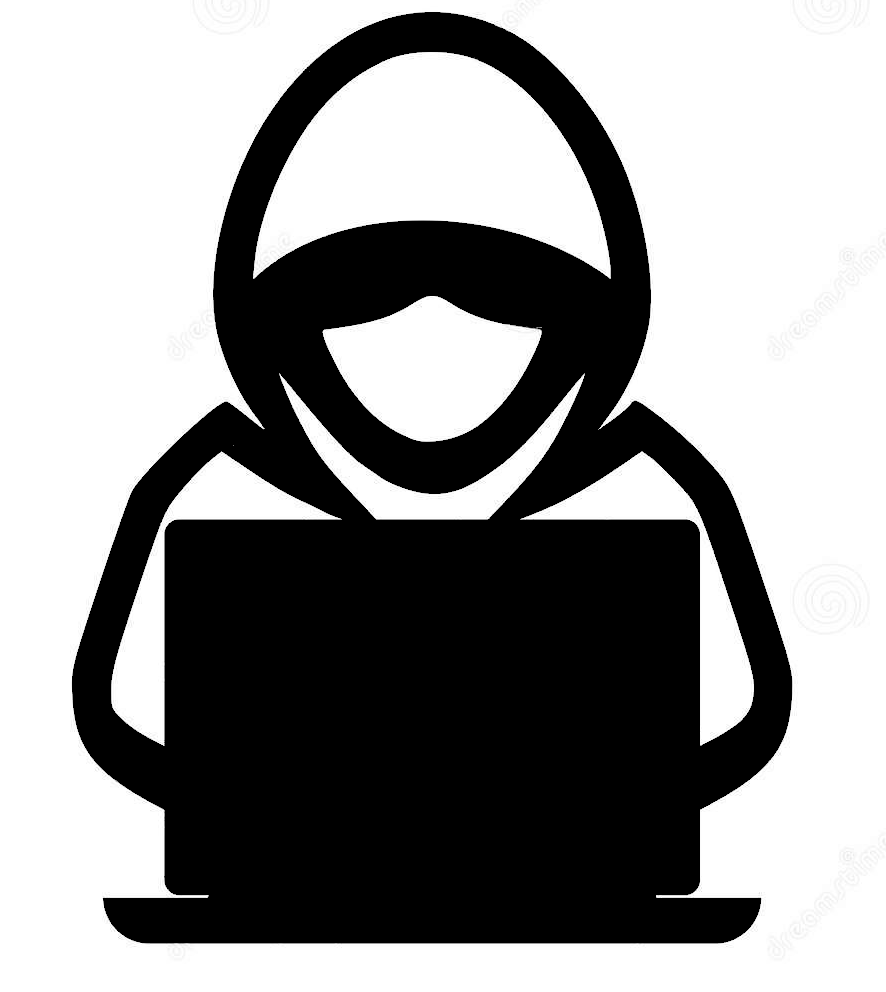
\includegraphics[width=5pt]{img/hacker.png}};

\end{tikzpicture}}

    \caption{\textsc{SGX-Spark} attacker model and collaborative structure scheme.\label{fig:sgx-spark-scheme}}
    \vspace{-19pt}
\end{wrapfigure}
\sgxspark~\cite{sgx-spark} builds on \textsc{SGX-LKL}.
It partitions the code of Spark applications to execute the sensitive parts inside SGX enclaves. 
Figure~\ref{fig:sgx-spark-scheme} depicts its architecture.
The engine deploys two collaborative Java Virtual Machines (JVM), one outside (Figure~\ref{fig:sgx-spark-scheme}, left) and one inside the enclave (Figure~\ref{fig:sgx-spark-scheme}, right) for the driver, and two more for each worker deployed in the cluster. 
Spark code outside the enclave accesses only encrypted data.
The communication between the JVMs is kept encrypted and is performed through the host OS shared memory.
\sgxspark provides a compilation toolchain, and it currently supports the vast majority of the native Spark operators, allowing to transparently deploy and run existing Spark applications into the SGX enclaves.
This is, the user must only compile the source code together with \textsc{SGX-Spark}'s and, as long as the operators used are supported by the framework, execution is seamlessly deployed inside the enclave with \emph{no} amendments to the vanilla Spark implementation.

\section{Cardiac Analysis} \label{sec:background:med}
The data streams used for the evaluation and the algorithms compiled with \textsc{SGX-Spark} belong to the medical domain and motivate the real need for confidentiality and integrity. 
As further explained in Chapter \ref{chap:architecture}, our use case contemplates a scenario where multiple sensors track the cardiac activity of different users.
The two most standard procedures for monitoring heart activity are electrocardiograms (ECG) and photoplethysmograms (PPG).
ECG-based systems measure the heart's electrical activity over time and is the chosen method by chest-based sensors~\cite{Tamura2018}.
PPG-based systems measure the variation of blood volume over time using LEDs and photodiodes.
Although less precise, PPGs are the chosen technique by all wrist-based cardiac monitoring sensors~\cite{Parak2015}.
In both cases, ECG and PPG based, we contemplate the usage of wearable sensors.
Wearable technologies are electronic devices that are incorporated into items which can comfortably be worn on the body~\cite{WearableDevices}.
Due to space and power constraints, these sensors' memory, computing power, and communication capabilities are limited.
As a consequence, to be embedded in a functional ecosystem, they rely on a gateway that forwards the information generated by the sensors to the cloud.
This environment is depicted in Figure~\ref{fig:wearable-enclave}.
% TODO: add figure illustrating!!
\begin{figure}[h!]
    \centering
    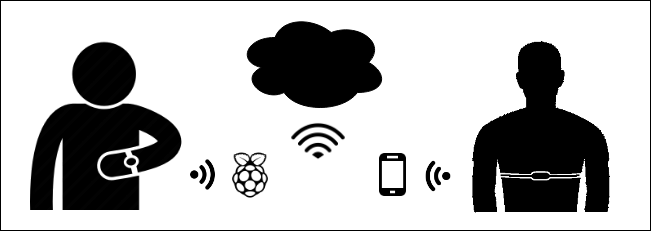
\includegraphics[width=.8\textwidth]{./img/wearable-ecosystem.png}
    \caption{\projName envisioned sensor ecosystem composed of: a wearable device, a gateway with internet connection, and the cloud were results are stored and processd.\label{fig:wearable-ecosystem}}
\end{figure}
%Both procedures lead to an approximation of R peaks' timestamps and the intervals between them (RR intervals). 
The generation of the approximated diagram (ECG or PPG) and the time measures are done inside the sensor.
Figure~\ref{fig:ecg-hrv} depicts a schematic representation of an ECG and the values streamed from the sensor to the gateway: R peak's timestamps and RR intervals. 
\begin{figure}[h!]
    \centering
    \resizebox{\linewidth}{!}{
\begin{tikzpicture}
    % Colors definition
    \pgfdeclaredecoration{single pulse}{initial}{
    \state{initial}[width=\pgfdecoratedinputsegmentlength]
    {%
        % Initial Line
        \pgfpathlineto{\pgfpoint{0.1*\pgfdecoratedinputsegmentlength}{0mm}}%    
        % P Peak
        \pgfpathsine{\pgfpoint{0.2\pgfdecorationsegmentlength}{0.15\pgfdecorationsegmentamplitude}}%
        \pgfpathcosine{\pgfpoint{0.2\pgfdecorationsegmentlength}{-0.15\pgfdecorationsegmentamplitude}}%
        % P - Q Line
        \pgfpathlineto{\pgfpoint{0.6\pgfdecorationsegmentamplitude}{0mm}}%
        % Q Valley
        \pgfpathsine{\pgfpoint{0.1\pgfdecorationsegmentlength}{-0.15\pgfdecorationsegmentamplitude}}
        \pgfpathcosine{\pgfpoint{0.01\pgfdecorationsegmentlength}{0.15\pgfdecorationsegmentamplitude}}%
        % R Peak
        \pgfpathsine{\pgfpoint{0.15\pgfdecorationsegmentlength}{\pgfdecorationsegmentamplitude}}%
        \pgfpathcosine{\pgfpoint{0.15\pgfdecorationsegmentlength}{-\pgfdecorationsegmentamplitude}}%
        % S Valley
        \pgfpathsine{\pgfpoint{0.15\pgfdecorationsegmentlength}{-0.5\pgfdecorationsegmentamplitude}}
        \pgfpathcosine{\pgfpoint{0.15\pgfdecorationsegmentlength}{0.5\pgfdecorationsegmentamplitude}}%
        % S to T line
        \pgfpathlineto{\pgfpoint{1.25\pgfdecorationsegmentamplitude}{0mm}}%
        % T Peak
        \pgfpathsine{\pgfpoint{0.8\pgfdecorationsegmentlength}{0.3\pgfdecorationsegmentamplitude}}%
        \pgfpathcosine{\pgfpoint{0.8\pgfdecorationsegmentlength}{-0.3\pgfdecorationsegmentamplitude}}%
        % Last Line
        \pgfpathlineto{\pgfpointdecoratedinputsegmentlast}%
    }
    \state{final}{}%
    }

    \fill[gray!10, draw=black] (-0.75, -0.75) rectangle (6.25, 1.75);
    \node at (-0.5, -0.5) {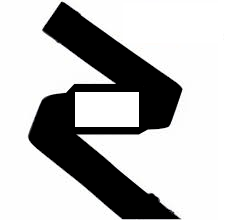
\includegraphics[width=10pt]{img/hrband.png}};
    %\node at (5.5, 1.5) {\textbf{\small{Sensor}}};

    \draw[->, dashed] (5.55,0) -- (6,0) node[pos=.5, anchor=north, xshift=-10pt] {\tiny{Time ($s$)}};
    \draw[->, dashed] (0,0) -- (0,1.25) node[anchor=south, xshift=10pt] {\tiny{Amplitude ($mV$)}};
    \draw[decoration={single pulse,amplitude=8mm,segment length=2mm},decorate] (0,0) -- (2,0);
    \draw[decoration={single pulse,amplitude=8mm,segment length=2mm},decorate] (2,0) -- (4,0);
    \draw[decoration={single pulse,amplitude=6mm,segment length=2mm},decorate] (4,0) -- (5.5,0);
    \draw[<->, dashed, thick] (0.55, 0.7) -- (2.5, 0.7);
    \draw[<->, dashed, thick] (2.55, 0.55) -- (4.35, 0.55);
    \node[align=center] at (0.5, 0.95) {\tiny{$\text{R}_0$}};
%    \node[align=center] at (2.2, 0.3) {\tiny{$\text{P}_1$}};
%    \node[align=center] at (2.45, -0.2) {\tiny{$\text{Q}_1$}};
%    \node[align=center] at (2.7, -0.55) {\tiny{$\text{S}_1$}};
%    \node[align=center] at (3.15, 0.38) {\tiny{$\text{T}_1$}};
    \node[align=center] at (2.5, 0.95) {\tiny{$\text{R}_1$}};
    \node[align=center] at (4.25, 0.8) {\tiny{$\text{R}_2$}};

    % Signal
    \fill[black] (6.5, 0) circle (0.05);
    \draw (6.75, -0.15) arc (-20:20:0.5);
    \draw (6.95, -0.25) arc (-30:30:0.5);
    \draw (7.15, -0.35) arc (-40:40:0.5);

    % Data file
    \node[align=center] at (9, 1.2) {\tiny{\textbf{\texttt{gateway://data/data\_file.csv}}}};
    \draw (7.45, -0.75) -- (7.45, 1) -- (10.5,1) -- (10.5, -0.5) to[out=180, in=0] (7.45, -0.75);
    \node[align=center] at (9, 0.2) {\tiny{\texttt{t}$\left(\text{R}_1\right)$, \xspace\texttt{t}$\left(\text{R}_1\right)$ - \texttt{t}$\left(\text{R}_0\right)$} \\ \tiny{\texttt{t}$\left(\text{R}_2\right)$, \xspace\texttt{t}$\left(\text{R}_2\right)$ - \texttt{t}$\left(\text{R}_1\right)$} \\ \tiny{\textbf{$\vdots$}}};
\end{tikzpicture}}

    \caption[Schematic representation of an ECG signal showing three normal beats.]{Schematic representation of an ECG signal showing three normal beats. A normal electrocardiogram can be broken down in three waves: a \textit{P wave} corresponding to the depolarization of the atria, a \textit{QRS complex} corresponding to the depolarization of the ventricles and a \textit{T wave} corresponding to the repolarization of the ventricle~\cite{Lilly2001}. From an ECG the sensor extracts and streams the R-peaks' timestamp and the time elapsed between them. \label{fig:ecg-hrv}}
\end{figure}

In our case, \projName focuses on the analysis of the Heart Rate Variability (HRV)~\cite{Camm1996}, that is, the analysis of the variation in the time intervals between heartbeats (a.k.a. RR intervals).
The HRV is of utmost importance since it has been shown to be a predictor for myocardial infarction~\cite{Kleiger1987,Bigger1992}.
With healthy individuals' heart rate (HR) averaging between 60 to 180 beats per minute (bpm), the average throughput per client is between 23 and 69 bytes per second.
%An interesting use case of RR processing, besides HR approximation, is the study of Heart Rate Variability (HRV). 
%HRV~\cite{hrv} is the variation in the time intervals between heartbeats and it has been proven to be a predictor of myocardial infarction.
Finally, despite \projName being specifically designed for streams with these data features, its modular design (as we later describe in Chapter \ref{chap:architecture}) makes it easy to adapt to other use-cases.
